\chapter{Testing \& Results}
\label{ch:testing_results}
\acresetall

In this chapter two tests are described and their results presented and
discussed. The two tests measure and compare the time performance in two common
stages for both the original implementation of BATMAN, and the extended version
proposed and implemented in this thesis.

\section{Test I - Initialization Phase}
The ``initialization phase'' is the setup phase between two or more nodes trying
to create a network. With the original implementation of BATMAN this phase only
consist of two stages; namely discovering a neighbor node, and deciding to add
the node as a direct link, or ``last-hop'' per BATMAN terminology, in its
routing table.

With the proposed design and implementation from this thesis, two more stages
are added. After the discovery, the authentication handshake stage and the
keystream sharing stage are conducted before the last stage where BATMAN adds
the node as a new direct link in its routing table.

The time measured here in this test is the time between the first discovery of a
new neighbor, until that node is added to the routing table.

\subsection{Hypothesis}
With the modified version of BATMAN proposed in this thesis, one should observe
a small extra delay in the setup of the network, compared to the original
BATMAN protocol. This extra delay should however, not be significantly higher,
i.e. it should be relatively constant and at no time should any linear increase
in delay be observed.

\subsection{Setup}
\begin{figure}[h]
	\centering
	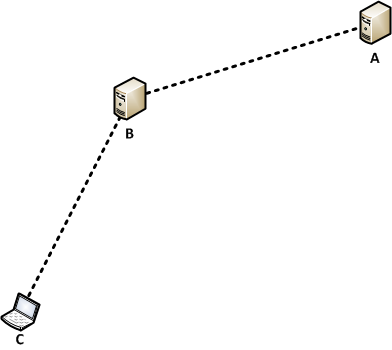
\includegraphics[width=0.5\textwidth]{images/setup_test_1.png}
	\caption{Physical network layout used in test 1. When using the modified version node B acts as the SP of the network}
	\label{fig:setup_test_1}
\end{figure}

Figure \ref{fig:setup_test_1} presents the setup of the test machines used to
conduct this first test. Node A and B are stationary boxes while node C is a
laptop. Their hardware specifications are described in Appendix
\ref{appendix:lab_setup}. The reasoning to use a different hardware for node C
is the need to create distance in the network, and that outside the ethernet
subnet for which the two other nodes were connected to, it would be easier to
use a laptop during setup. In the next test, this laptop is yet again moved
further away.

An important feature to notice about how these nodes were set up is that node A
and C are outside each other transmitting range, meaning they need an
intermediate node to route their packets to and from each other. Node B is
conveniently placed with almost equal distance to each of the two other nodes.

The landscape the nodes are setup in is a typical office landscape, with varying
obstructing materials such as concrete, wood, and glass. A more ideal setup
would naturally be outdoors, as the network is intended for, but with the lack
of mobile nodes and time this became out of the option.

\subsection{Procedure}
In order to get the same behaviour each run for the modified version, each run
had to be run discretely, i.e. after each run the daemon was shut down and
restarted. This way each run will include all four stages explained above:
discovery, authentication handshake, keystream material sharing, and routing
table update. This was also done on the original implementation, even though
there are no authentication steps in between, but in order to have the exact
same procedure each time.

For each run, these steps were followed:
\begin{enumerate}
  \item Start Node A and C
  \item Wait and make sure both nodes are stable
  \item Start Node B
  \item When both node A and C are discovered and added to routing table kill
  all daemons
  \item Record the log from node B
\end{enumerate}
These steps were taken 10 times in order to have a reasonable data set and
average. Then for each of the 10 logs, record the time between the first routing
announcement received from a node, until both nodes have been added to the
routing table.

\section{Test II - Route Convergence}
The next test is to check how quick route convergence the protocols deliver when
a path between nodes in the network changes. As with the previous test, a
node running the original protocol needs to discover a new direct neighbor and
add it to its routing table. In addition, it will have to receive not only the
neighbors own routing announcements, but also routing announcements it has
forwarded on behalf of its own direct neighbors. When this happens, the node
receiving these re-broadcasts determines new routes to possibly new nodes -
adding them to its routing table.

Additionally, nodes using the modified BATMAN protocol needs to share
their keystream material with their new direct neighbor before adding that
neighbor in their routing table. When this has happened, any re-broadcasted
routing announcements from that neighbor is accepted and paths to those nodes
are updated, or added if new nodes. Note also that no authentication handshake
or sharing of certificates are mentioned, as they are assumed to have been
shared prior to this route change.

\subsection{Hypothesis}
As before, a small and relatively constant (mathematical term) extra delay is
expected when running the modified version of the protocol compared to running
the original. As the keystream material sharing only occurs between the direct
neighbors, it should only happen once during one run and not for each of the new
nodes added by the path through the direct neighbor - i.e. there should be no
linear increase in convergence time even if multiple new nodes are added to the
routing table with paths through a new neighbor.

\subsection{Setup}
\begin{figure}[h]
	\centering
	\subfloat[1st Position]{\label{fig:test_2_1}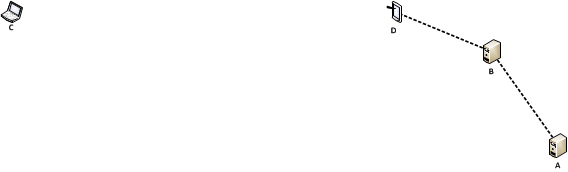
\includegraphics[width=\textwidth]{images/setup_test_2_1.png}}
	\\
	\subfloat[2nd Position]{\label{fig:test_2_2}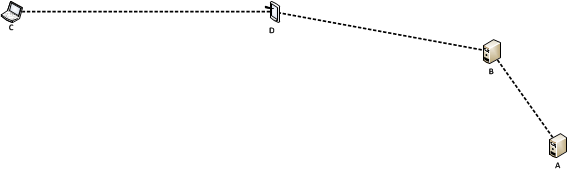
\includegraphics[width=\textwidth]{images/setup_test_2_2.png}}
	\caption{Physical network layout used in test 2. The Laptop (node C) is moved further out of range and is periodically rejoining the network when a Tablet Pc (node D) is moved within range. When using the modified version node B acts as the SP of the network}
	\label{fig:setup_test_2}
\end{figure}

For this test a new mobile node was needed. As Figure \ref{fig:setup_test_2}
shows the Laptop, or node C, from the previous test is moved much further away,
so far in fact the newly added Tablet Pc, node D, needs to place itself with
approximately the same distance to node B as to node C in order for node C to
take part in the network.

Node A and B is positioned at the same place as in the previous test, in the
same office landscape. The line of sight is, however better between node B and
D, and between D and C. Their line of sighs are only obstructed by a single wall
with huge windows.

\subsection{Procedure}
With this test running each of the 10 iterations discretely would be too time
consuming, because it would have meant that the Laptop (node C) would have to be
physically moved inside the transmitting range of node B for each run. Instead
the laptop was only started within the range of the other nodes, in order to be
authorized and share certificates with the other nodes (only node B and D was
necessary) and then moved to its position long outside the transmitting range of
the rest of the network. After this ``initial setup'' plus some minutes to
clear the neighbor lists, these steps were followed:
\begin{enumerate}
  \item Walk node D in between node B and C
  \item Wait until the whole network has stabilized
  \item Walk node D back out of node C's range
  \item Wait until BATMAN has cleared node D from other nodes routing tables,
  and node D has cleared all other nodes from its routing table
  \item If modified version is used, make also sure node D is removed from the
  \ac{NL} (should be before routing tables are cleared)
\end{enumerate}
These steps were repeated 10 times for both implementations. The records used
from this test are from the logs of node C. The convergence times measured
are the time between each time a new neighbor (node D) is discovered by BATMAN,
and until a path to the furthermost node (A) is added to the routing table.


\section{Results}
In this section the results from the two tests above are presented and discussed
in terms of how they perform compared to the hypotheses. In both tests there
were only a dataset of 10 trials, which given the variance shown below does not
provide a statistical significant result. However, the first test shows good
indication that the modified protocol behaves as expected, while the results
from the seconds test are more ambiguous.

\subsection{Initialization Phase}
Figure \ref{fig:results_test_1} presents the first test's results for both the
original and modified version of BATMAN. The two graphs shows the time in
seconds on the y-axis and the trial/run number on the x-axis. The two colored
lines on the graps shows the results from first neighbor discovery until the
first neighbor is added to routing table (green line) and until both nodes are
added to the routing table (red line).

\begin{figure}[h]
	\centering
	\subfloat[Original B.A.T.M.A.N.]{\label{fig:test_1_original}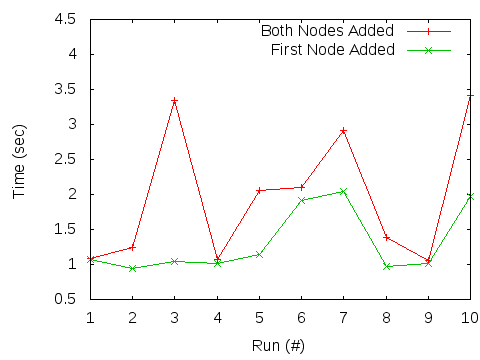
\includegraphics[width=0.5\textwidth]{images/test_1_original.png}}
	\subfloat[Modified B.A.T.M.A.N.]{\label{fig:test_1_secure}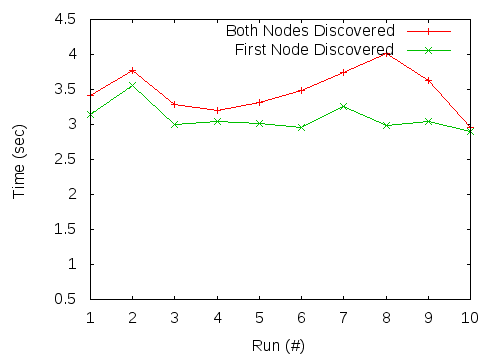
\includegraphics[width=0.5\textwidth]{images/test_1_secure.png}} 
	\caption{In a network of three nodes, the time spent by the \ac{SP} from its first neighbor discovery and until both neighbors are added to its routing table.}
	\label{fig:results_test_1}
\end{figure}

The results from the original protocol, shown in Figure
\ref{fig:test_1_original}, shows high variance in the time needed to add one and
two nodes to the routing table. For 7 out of 10 ``first nodes'' the time needed
is relatively equal, being about one second. For both nodes to be added however,
there are much more variance - variying from the best possible time, i.e. equal
to adding one node, and up above 3 times longer than adding one node. As this is
from the original implementation of BATMAN, this thesis will not try to explain
why this behaviour is observed, nor does the writer know exacly why either.

Figure \ref{fig:test_1_secure} shows the results from the modified version
proposed in this thesis. These results indicates that the behaviour of the
modified version seems to correlate with the behaviour expected from the
hypothesis. A seemingly constant of about two seconds seems to be added to the
process of adding both nodes to the routing table. 

Another interesting observation is that the time variance seems to be much less
from that of the original version. This might be because the authentication
handshake and the keystream sharing happens in a separate thread from the
regular BATMAN operations, meaning the BATMAN protocol continously receives
routing announcements to process while the \ac{AM} handles its part. The idea
being that while the \ac{AM} thread runs the BATMAN thread ``gets ready'' to do
its part of the job.

\subsection{Route Convergence}
The results of the second test is shown in Figure \ref{fig:results_test_2}. In
this figure, the axes are the same as in the figures above: y-axis shows the
time in seconds, and the x-axis shows the trial run. The red line shows the
performance of the original implementation, while the green line shows the
modified.

\begin{figure}[h]
	\centering
	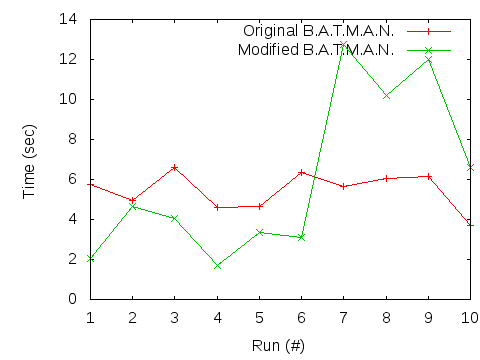
\includegraphics[width=0.8\textwidth]{images/test_2.png}
	\caption{Routing path convergence time observed by a distant source node to another sink node in the network. The source node is only sporadically connected to the network through a mobile intermediate node.}
	\label{fig:results_test_2}
\end{figure}

As indicated earlier, this test's results are somewhat unclear. While the
results using the original implementation seems relatively uniform, with only
about 1 second variance, the results from the modified implementation is highly
irregular.

Looking through the logs from this test one thing become apparent. With
different hardware on the different nodes in the network, their wireless cards
send at different strengths meaning while one node can receive packets from a
``stronger node'', the packets sent might not be received by the other nodes.

The BATMAN protocol messages (routing announcements) are sent quite often,
depending on the number of re-broadcasts being sent, meaning the time from when
a node is within transmitting range and until its broadcasts are received by
nodes within its transmitting range will be quite short. The \ac{AM} messages
however, was mostly tested in an ideal environment where most packets were
received, so this was not properly accounted for. Therefore, if a routing
announcement from a ``stronger node'' is received by a ``weaker node'', the
weaker node might send its keystream material without the other node receiving
it.

Re-transmitting mechanisms based on guessing that the receiving node has not
received the \ac{AM} messages are in place, but as the mechanism wait until it
beleives the other node has not received, instead of knowing it instantly. This
can of course be managed adding ACK'ing to each \ac{AM} message, which was not
added initially because of the wish to minimize overhead. This however, might
have to be re-evaluated.

Another thing to notice is how multiple trial runs using the modified version
actually performed better than the original version. This is impossible to
explain talking about the design and implementations themselves, but is probably
most accuratly explained in the terms of external environment.

In this test, one major factor is the movement of the Tablet Pc, or node D. This
movement is not perfect, and will vary in speed, timing, and accurate position
for each run. As self-generated routing announcements is only generated every
one second, a difference in almost two seconds can be seen based on the
difference in distance each run. Also, the original implementation only starts
its whole neighbor discovery after an original (self-generated/produced) routing
annoucement is received from a new neighbor. The \ac{AM} is triggered on the
first routing annoucement received from that new neighbor, even if that
annouement is a re-broadcast from another node in the new neighbor's network.
